\documentclass{beamer}
%
% Choose how your presentation looks.
%
% For more themes, color themes and font themes, see:
% http://deic.uab.es/~iblanes/beamer_gallery/index_by_theme.html
%
\mode<presentation>
{
  \usetheme{default}      % or try Darmstadt, Madrid, Warsaw, ...
  \usecolortheme{default} % or try albatross, beaver, crane, ...
  \usefonttheme{serif}  % or try serif, structurebold, ...
  \setbeamertemplate{navigation symbols}{\insertframenumber/\inserttotalframenumber}
  \setbeamertemplate{caption}[numbered]
  
} 

\usepackage[english]{babel}
\usepackage[utf8]{inputenc}
\usepackage[font=scriptsize,labelfont=bf]{caption}

\title[APC 524 Design Review]{Tabulation of Chemical Source Terms for Turbulent Combustion Simulations}
\author{Emmet Cleary \\
Daniel Floryan \\
Jeffry Lew \\
Bruce Perry \\
Emre Turkoz} 
\date{January 8, 2014}

\begin{document}

\begin{frame}
  \titlepage
\end{frame}

% Uncomment these lines for an automatically generated outline.
%\begin{frame}{Outline}
%  \tableofcontents
%\end{frame}

\section{Introduction}
\begin{frame}{Introduction}
Flamelet Modeling for Tubulent Combustion Simulations:
\begin{figure}
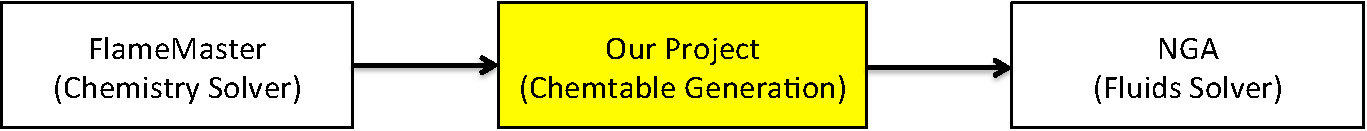
\includegraphics[width=\textwidth]{scope.pdf}
\end{figure}
%\vskip 2mm
Key Data Processing Capabilities:
\begin{itemize}
\item Sorting
\item Monotonicity checking
\item Convolution
\item Interpolation
\end{itemize}
\vspace{12pt}
\end{frame}


\section{Inputs and Outputs}
\begin{frame}{Program Structure}
Inputs:
\begin{itemize}
\item chemtable\_inputs (text file) %containing input options
\item flamelet(.kg) data files %: stored in a directory specified in the input file
\end{itemize}


Outputs:
\begin{itemize}
\item Processed chemical source term data (text file)
\item Plot of progress variable vs. temperature
\item Contour plots of the chemical source term
\end{itemize}

\vspace{12pt}
Tools used:
\begin{itemize}
\item SWIG $\rightarrow$ Interface C++ and Python\\
\item Git $\rightarrow$ Version control\\
\item Doxygen $\rightarrow$ Documentation\\ %% Remove ?
\item Python Unittest $\rightarrow$ Automated testing
\end{itemize}

\end{frame}


%%%%%%%%%%%%%%%%%%%%%%%%%%%%%%%%%%%%%%%%%%%%%%%%%%%%%%%%%%%%%%%%%%%%%%%%%%%%%%%%
%%%%%%%%%%%%%%%%%%%%%%%%%%%%%%%%%%%%%%%%%%%%%%%%%%%%%%%%%%%%%%%%%%%%%%%%%%%%%%%%
\section{Flowcharts}
%%%%%%%%%%%%%%%%%%%%%%%%%%%%%%%%%%%%%%%%%%%%%%%%%%%%%%%%%%%%%%%%%%%%%%%%%%%%%%%%
%%%%%%%%%%%%%%%%%%%%%%%%%%%%%%%%%%%%%%%%%%%%%%%%%%%%%%%%%%%%%%%%%%%%%%%%%%%%%%%%
\subsection{Progress Variable}
\begin{frame}{Progress Variable}
\begin{figure}
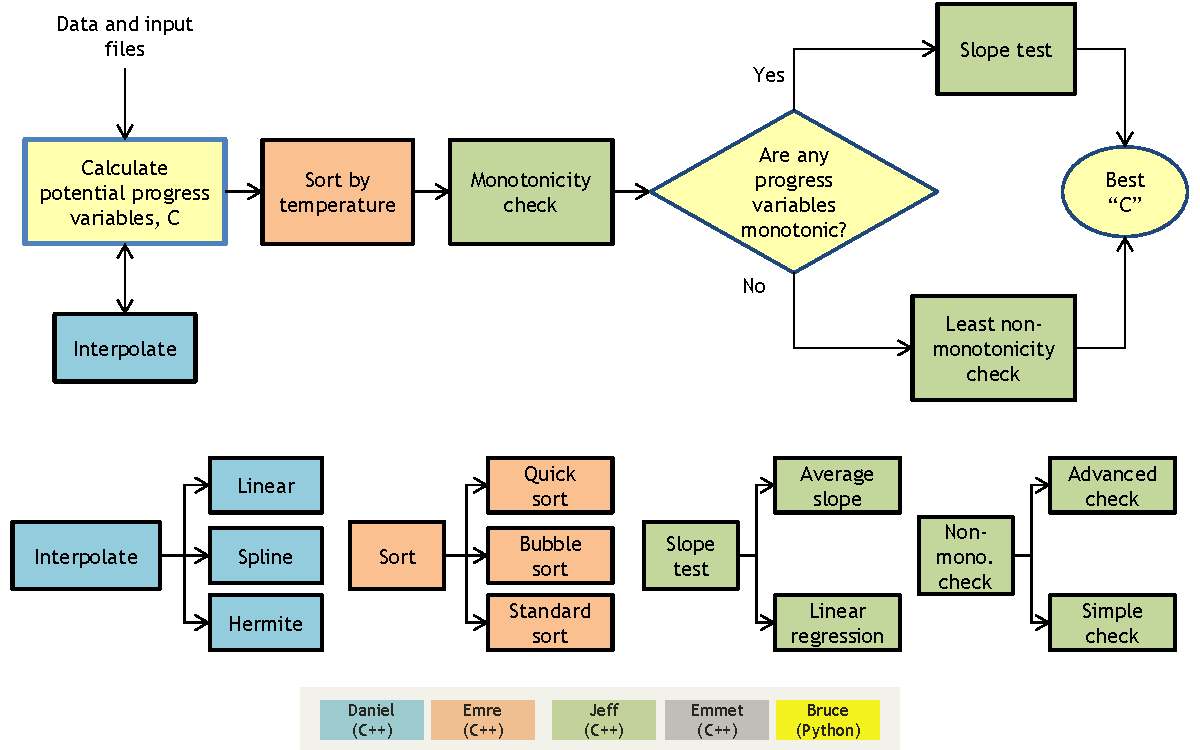
\includegraphics[width=\textwidth]{diagram_1_shortened_v3.pdf}
\end{figure}
\end{frame}

%%%%%%%%%%%%%%%%%%%%%%%%%%%%%%%%%%%%%%%%%%%%%%%%%%%%%%%%%%%%%%%%%%%%%%%%%%%%%%%%
\subsection{Table Generation}
\begin{frame}{Table Generation}
\begin{figure}
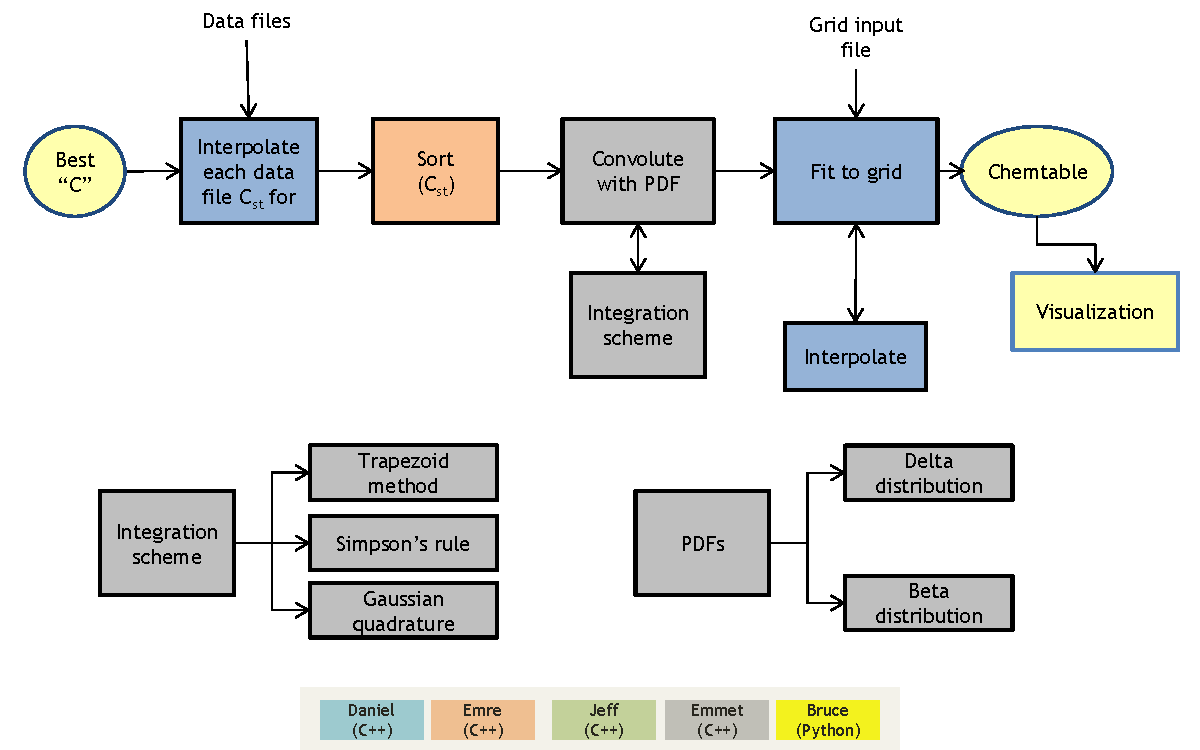
\includegraphics[width=\textwidth]{diagram_2_shortened_v3.pdf}
\end{figure}
\end{frame}


%%%%%%%%%%%%%%%%%%%%%%%%%%%%%%%%%%%%%%%%%%%%%%%%%%%%%%%%%%%%%%%%%%%%%%%%%%%%%%%%
%%%%%%%%%%%%%%%%%%%%%%%%%%%%%%%%%%%%%%%%%%%%%%%%%%%%%%%%%%%%%%%%%%%%%%%%%%%%%%%%
\section{Modules}
%%%%%%%%%%%%%%%%%%%%%%%%%%%%%%%%%%%%%%%%%%%%%%%%%%%%%%%%%%%%%%%%%%%%%%%%%%%%%%%%
%%%%%%%%%%%%%%%%%%%%%%%%%%%%%%%%%%%%%%%%%%%%%%%%%%%%%%%%%%%%%%%%%%%%%%%%%%%%%%%%

\subsection{Python: User Interface and Wrapper}
\begin{frame}{Python: User Interface and Wrapper}
Python files:
%\begin{itemize}
\begin{itemize}
\item chemtable\_io.py: Main program run by user: processes inputs, calls findprogvar.py and C++ functions, and generates ouput %%MAKE THESE TITLES BOLD OR ITALIC
\item findprogvar.py: contains function that determines the best progress variable, calls C++ functions
\item iofuncs.py: contains functions used by the above for text processing
\item combinations.py: contains helper functions used by findprogvar.py
\end{itemize}
\vspace{12pt}
User specified inputs stored in a Python dictionary
%\item chemtable_io.py:
%\item findprogvar.py:
%\item iofuncs.py:
%\item combinations.py:
%\end{itemize}


\end{frame}

%%%%%%%%%%%%%%%%%%%%%%%%%%%%%%%%%%%%%%%%%%%%%%%%
\subsection{Python/C++ Interface Using SWIG}
\begin{frame}{Python/C++ Interface Using SWIG}

\begin{figure}
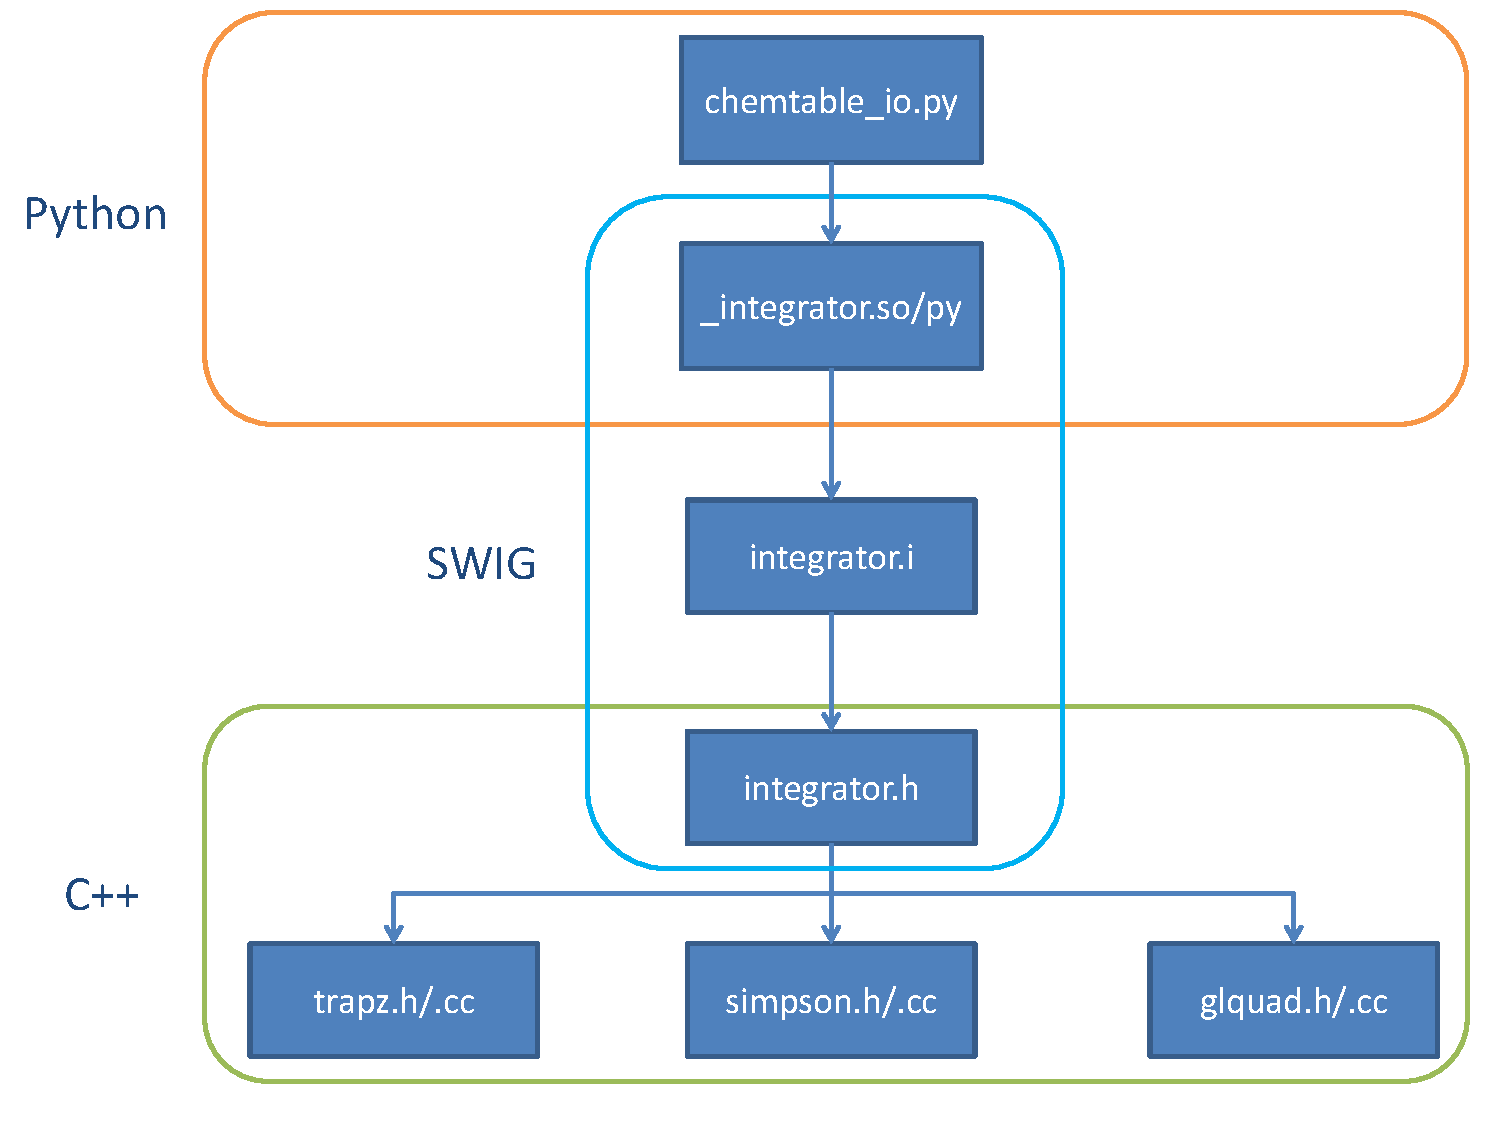
\includegraphics[width=\textwidth]{python_swig_c++.pdf}
\end{figure}


\end{frame}

%%%%%%%%%%%%%%%%%%%%%%%%%%%%%%%%%%%%%%%%%%%%%%%%
%%%%%%%%%%%%%%%%%%%%%%%%%%%%%%%%
%\subsection{Modules: Matrix/Matrix3D/Matrix4D}
%\begin{frame}{Modules: Matrix/Matrix3D/Matrix4D}
%Matrix.h/.i, Matrix3D.h/.i, Matrix4d.h/.i
%\begin{itemize}
%\item Matrix.cc
%\item Matrix3D.cc
%\item Matrix4D.cc
%\end{itemize}

%\vspace{10pt}
%Constructors:
%\begin{itemize}
%\item Matrix(int dim1, int dim2)
%\item Matrix3D(int dim1, int dim2, int dim3)
%\item Matrix4D(int dim1, int dim2, int dim3, int dim4)
%\end{itemize}

%\end{frame}

%%%%%%%%%%%%%%%%%%%%%%%%%%%%%%%%%%%%%%%%%%%%%%%%%%%%%%%%%%%%%%%%%%%%%%%%%%%%%%%%
\subsection{Documentation}
\begin{frame}{Documentation: Doxygen}
\begin{figure}
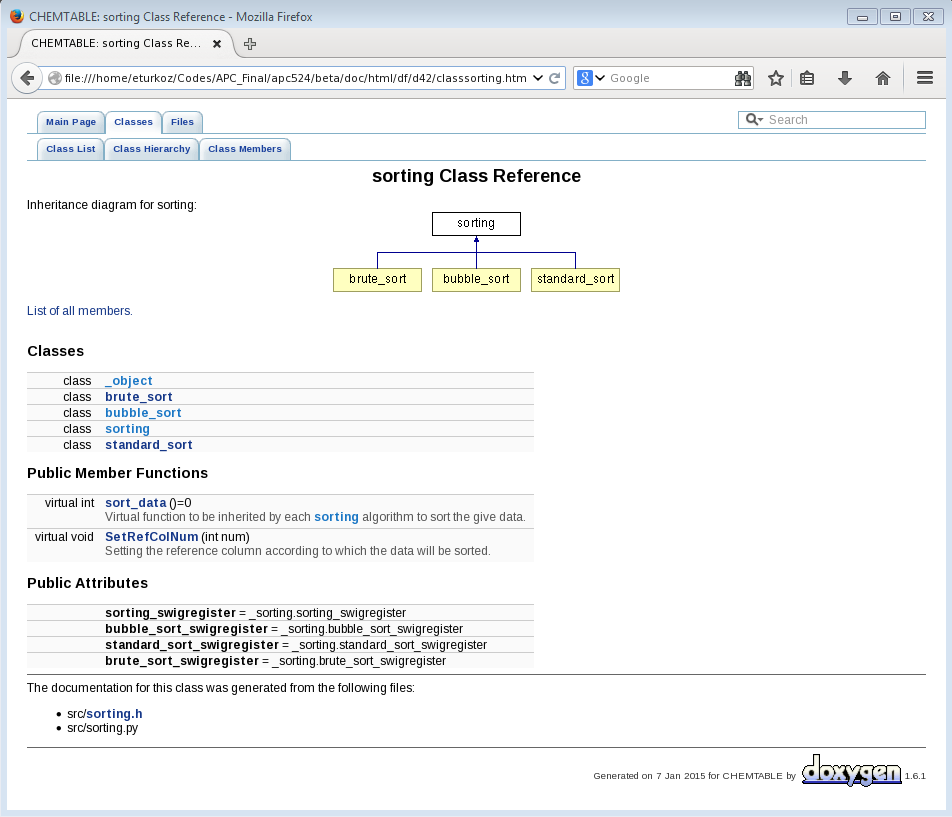
\includegraphics[scale=0.35]{doxygen.png}
\end{figure}

\end{frame}


\section{Conclusions}

\begin{frame}{Conclusions}
We are better friends now.


\end{frame}







\end{document}
